% Using KOMA Script document style
% Font size setting and
% option to skip empty lines as new paragraphs
\documentclass[10pt,a4paper]{article}
% Packages without Options
\usepackage{
	algorithm,
	algpseudocode,
	amsfonts,
	amssymb,
	appendix,
	array,
	booktabs,
	enumitem,
	float,
	footnote,
	gensymb,
	geometry,
	graphicx,
	interval,
	karnaugh-map,
	lipsum,
	listings,
	longtable,
	makecell,	mathtools,
	minted,
    nicematrix,
	parskip,
	pdfpages,
	pgfkeys,
	pgfplots,
    sectsty,
	subcaption,
	tablefootnote,
	textcomp,
	tikz,
    titlecaps,
	venndiagram,
	wrapfig,
	wrapfig,
	xcolor
}

% Packages with Options

\usepackage[framemethod=tikz]{mdframed}
\usepackage[colorlinks,linkcolor=cyan, citecolor=cyan, urlcolor=cyan]{hyperref}
\usepackage[labelfont=bf,textfont=it,labelsep=period]{caption}
\usepackage[RPvoltages]{circuitikz}
\usepackage[british]{babel}
\usepackage[nameinlink,noabbrev]{cleveref}

\definecolor{mintedbackground}{rgb}{0.97,0.97,0.97}

\setminted[cpp]{
bgcolor=mintedbackground,
    linenos=true,
    breaklines=true,}

\setminted[js]{
bgcolor=mintedbackground,
    linenos=true,
    breaklines=true,}

\setminted[python]{
bgcolor=mintedbackground,
    linenos=true,
    breaklines=true,}
    
% Enforce title case for section
\allsectionsfont{\titlecap}

% \lstset{basicstyle=\footnotesize\ttfamily,breaklines=true}

\linespread{1.5}



% Package: Interval
% Sets the style of mathematical intervals
\intervalconfig{
soft open fences, separator symbol=,,
}

% Package: Geometry
% Sets the page margins
\geometry{
    a4paper,
    left=32mm,
    right=22mm,
    top=22mm,
    }
	
% Creates a proper caption name for algorithms
\newcommand{\algorithmautorefname}{Algorithm}
\newcommand{\listingautorefname}{Listing}
\algrenewcommand{\algorithmiccomment}[1]{\texttt{// #1} }
% Creates a numbered environment for Theorems
\newtheorem{theorem}{Theorem}

% Redefine the implication arrow to be a simple, thin arrow instead of the default, thick arrow
\renewcommand{\implies}{\rightarrow}

% Create a new command for the set complement to make my logical statements easier to read
\newcommand{\compl}{\overline}

% Creates commands for combinatorics nCr and nPr
\newcommand{\nCr}[2]{\,_{#1}C_{#2}} % nCr
\newcommand{\nPr}[2]{\,_{#1}P_{#2}} % nPr

% Package: tikz
% Loads libraries for drawing automata, 
\usetikzlibrary{automata,positioning,shadows,arrows, shapes.gates.logic.US, calc}

% Creates a command to create a button shape
\newcommand*\keystroke[1]{%
  \tikz[baseline= (key.base)]
    \node[%
      draw,
      fill=white,
      drop shadow={shadow xshift=0.25ex,shadow yshift=-0.25ex,fill=black,opacity=0.75},
      rectangle,
      rounded corners=2pt,
      inner sep=1pt,
      line width=0.5pt,
      font=\scriptsize\sffamily
    ] (key) {#1\strut};
}

% Package: pgfplot
% Sets the global options for PGF Plots
\pgfplotsset{compat=newest}

% Package: tikz
% Flowchart Shapes
\tikzstyle{startstop} = [rectangle, rounded corners, minimum width=3cm, minimum height=1cm,text centered, draw=black, fill=red!30]
\tikzstyle{io} = [trapezium, trapezium left angle=70, trapezium right angle=110, minimum width=3cm, minimum height=1cm, text centered, draw=black, fill=blue!30]
\tikzstyle{process} = [rectangle, minimum width=3cm, minimum height=1cm, text centered, draw=black, fill=orange!30]
\tikzstyle{decision} = [diamond, minimum width=3cm, minimum height=1cm, text centered, draw=black, fill=green!30]
\tikzstyle{arrow} = [thick,->,>=stealth]

% Disable Minted syntax error highlights (red boxes)
\AtBeginEnvironment{minted}{%
  \renewcommand{\fcolorbox}[4][]{#4}}


\graphicspath{{images/}}

\title{CM1025: Fundamentals of Computer Science \\ Summary}
\author{Arjun Muralidharan}

\begin{document}

\maketitle
\newpage
\tableofcontents
% \listoffigures
% \listoftables
% \listoflistings
% \listofalgorithms

\newpage
\renewcommand{\subsubsectionautorefname}{section\negthinspace}
\section{Propositional Logic}
\begin{mdframed}
\textbf{Learning Outcomes}
\begin{itemize}[label={\( \checkmark \)}]
\item Define propositional logic and learn some of its properties 
\item Give some examples of domains where 
	propositional logic is used  
\item Defining a proposition in mathematical context and distinguish examples of sentences considered as propositions and other that are not propositions 
\item Learn how propositional variables help to simplify notations 
\item Learn how we can build a truth table and give an example of how it works 
\item Practice how to build compound statements using logical operators and take into consideration the order of precedence of the operators 
\item Define truth sets and learn some examples of truth sets for some compound propositions 
\item Define what is an implication and equivalence, what are their properties and build their truth table 
\item Learn some important laws of propositional logic including De Morgan’s laws, and practice their use in building a reasoning, and proving equivalence
\end{itemize}
\end{mdframed}
\subsection{Connectives}
A \textbf{proposition} is a declarative sentence that is either true or false, but not both. We use \textbf{propositional} or \textbf{sentential} variables such as \(p,q,r,s \ldots \) to represent propositions. The \textbf{truth value of a proposition} is denoted by \textbf{T} or \textbf{F}. The simplest form of a proposition is an \textbf{atomic proposition}. Propositions can be placed in relation to one another using \textbf{connectives}.

\subsubsection{Negation}
Let \( p \) be a proposition. The \emph{negation} of \(p\) is stated as \[\mathbf{\neg p}\]
and proposes that ``It is not the case that \(p\)''.

The proposition \(\neg p\) is read ``not \(p\)''. The truth value of the negation of \(p, \neg p, \) is the opposite of the truth value of \(p\).

\subsubsection{Conjunction}
Let \(p\) and \(q\) be propositions. The \emph{conjunction} of \(p\) and \(q\), is denoted as \[\mathbf{p \wedge q }\] and proposes that ``\(p\) and \(q\)''.

The \emph{conjunction} \(p \wedge q\) is true when both \(p\) and \(q\) are true and is false otherwise.

\subsubsection{Disjunction}
Let \(p\) and \(q\) be propositions. The \emph{disjunction} of \(p\) and \(q\), denoted as \[\mathbf{p \vee q }\] is the statement ``\(p\) or \(q\)''.

The \emph{disjunction} \(p \vee q\) is false when both \(p\) and \(q\) are false and is true otherwise. This is an \textbf{inclusive or}, which means that the disjunction is true if at least one of the propositions is true, or both are true.

\subsubsection{Conditional Statements \& Implication}
Let \( p \) and \( q \) be propositions. The \emph{conditional statement} \[
p \implies q	
\]
is the proposition ``if \( p \), then \( q \).'' The conditional statement \( p \implies q \) is false when \( p \) is true and \( q \) is false, and true otherwise. In the implication \( p \implies q \), \( p \) is the \emph{hypothesis} (or \emph{antecedent} or \emph{premise}) and \( q \) is called the \emph{conclusion} (or \emph{consequence}).

The implication does not express causality in discrete mathematics. It only covers the truth value of the statement. It can also be read as:

\begin{enumerate}
	\item ``\( p \) is sufficient for \( q \) ''
	\item ``a necessary condition for \( q \) is \( p \) ''
	\item ``\( q \) unless \( \neg p \) ''
	\item ``\( q \) whenever \( p \) ''
\end{enumerate}

\subsubsection{Exclusive Or}

Let \(p\) and \(q\) be propositions. The \emph{exclusive or} of \(p\) and \(q\), denoted as \[ \mathbf{p \oplus q }\] is the statement ``either \(p\) or \(q\), but not both''.

The \emph{exclusive or} \(p \oplus q\) is true when exactly one of \(p\) and \(q\) is true and false otherwise. In other words, \( p \) and \( q \) may never have the same truth value.  

\subsubsection{Biconditional}
Let \(p\) and \(q\) be propositions. The \emph{biconditional statement} \[ \mathbf{p \leftrightarrow q } \] is the proposition ``\(p\) if and only if \(q\)''.

The biconditional statement \(p \leftrightarrow q\) is true when \(p\) and \(q\) have the same truth values, and is false otherwise.

\subsection{Truth Tables}
A truth table evaluates the truth values for propositions and connectives systematically. When given a compound proposition, a truth table can be used to evaluate the atomic propositions step-by-step and arrive at the correct truth value for the compound proposition.

\begin{table}[H]
\centering
\caption{Truth table for basic connectives}\label{tab:truth}
\begin{tabular}{@{}>{\bfseries}c>{\bfseries}cccccc@{}}
\toprule
 \( \mathbf{p} \) & \( \mathbf{q} \) & \(p \wedge q\) & \(p \vee q\) & \(p \oplus q\) & \(p \implies q\) & \(p \leftrightarrow q\)  \\ \midrule
 T & T & T & T & F & T & T \\
 T & F & F & T & T & F & F \\
 F & T & F & T & T & T & F \\
 F & F & F & F & F & T & T \\
  \bottomrule
\end{tabular}
\end{table}
Truth values can also be denoted using binary bits, i.e.~T is 1 and F is 0. When constructing a truth table, the number of rows is \(2^n\) where n is the number of propositions involved. So compound proposition involving 3 atomic propositions \(p, q, r\) has \(2^3 = 8\) rows.
Further, The the first column (e.g.~\(p\)) is constructed with all true values for the first half, and false values for the second half, the second (\(q\)) is true for the first 2 rows and false for next two rows, and the third is true for the first row and false for the second row of the table, and then this pattern repeats down the table for \(p, q\) and \(r\).

The universal and existential quantifications \( \forall \) and \( \exists \) are described in \autoref{ssub:quantifiers}.

\subsection{Precedence of Logical Operators}
Logical operators have an order of precedence as follows. \[
\forall \quad \exists \quad \neg \quad \wedge \quad \vee \quad \implies \quad \leftrightarrow
\]
\subsection{Propositional Equivalences}\label{ssec:equiv}
\begin{enumerate}
	\item \textbf{Tautology:} A compound proposition that is always true, no matter the truth values of the individual propositions
	\item \textbf{Contradiction:} A compound proposition that is always false, no matter the truth values of the individual propositions. This is called \textbf{inconsistent}.
	\item \textbf{Contingency:} A compound proposition that is true for at least one scenario of truth values. This is called \textbf{consistent}. All tautologies are consistent by definition.
\end{enumerate}

% TODO: Add contrapositive comment to equivalences table

\subsection{Logical Equivalence}
Compound propositions that have the same truth value in all possible cases are called \textbf{logically equivalent}. In other words, if \(p \leftrightarrow q\) is a tautology, then \(p \equiv q\).

Logical equivalence can be proved using truth tables.

\subsection{De Morgan's Laws}
\begin{gather*}
\neg (p \wedge q) \equiv \neg p \vee \neg q  \tag{De Morgan's First Law} \\
\neg (p \vee q) \equiv \neg p \wedge \neg q \tag{De Morgan's Second Law}
\end{gather*}
\subsection{Special equivalences}
\subsubsection{Conjunction-Disjunction} The \textbf{conditional-disjunction equivalence} allows us to replace conditional statements with disjunctions. This is especially useful to convert a conditional to a form that can then be transformed using De Morgan's laws.

\begin{gather*}
p \implies q \equiv \neg p \vee q
\end{gather*}

\subsubsection{Contrapositive}The \textbf{contrapositive} of a conditional statement is equivalent to the original conditional statement and is defined as follows.
\begin{gather*}
p \implies q \equiv \neg q \implies \neg p
\end{gather*}

\subsection{Summary of Logical Equivalences}
\begin{table}[H]
\centering
\caption{Summary of Equivalence Laws}\label{tab:identlaws}
\def\arraystretch{1.4}
\begin{tabular}{p{0.4\textwidth}p{0.4\textwidth}}
\toprule
Name  & Equivalence \\ \midrule
\textbf{Identity Laws} & \(p \wedge \mathbf{T} \equiv p\) \\
\textbf{} & \(p \vee \mathbf{F} \equiv p\) \\\midrule
\textbf{Domination Laws} & \(p \vee \mathbf{T} \equiv \mathbf{T}\) \\
\textbf{} &  \(p \wedge \mathbf{F} \equiv \mathbf{F}\) \\\midrule
\textbf{Idempotent Laws} & \( p \vee p \equiv p \) \\
\textbf{} &  \(p \wedge p \equiv p\)  \\\midrule
\textbf{Double Negation Law} & \(\neg(\neg p) \equiv p\) \\\midrule
\textbf{Commutative Laws} & \( p \vee q \equiv q \vee p \) \\
\textbf{} & \(p \wedge q \equiv q \wedge p \) \\\midrule
\textbf{Associative Laws} & \( (p \vee q) \vee r \equiv p \vee(q \vee r) \) \\
\textbf{} & \((p \wedge q) \wedge r \equiv p \wedge(q \wedge r)\)  \\\midrule
\textbf{Distributive Laws} & \(p \vee(q \wedge r) \equiv(p \vee q) \wedge(p \vee r)\) \\
\textbf{} & \(p \wedge(q \vee r) \equiv(p \wedge q) \vee(p \wedge r)\) \\ \midrule
\textbf{De Morgan's Laws} & \(\neg(p \wedge q) \equiv \neg p \vee \neg q\) \\
\textbf{} & \(\neg(p \vee q) \equiv \neg p \wedge \neg q\) \\\midrule
\textbf{Absorption Laws} & \(p \vee(p \wedge q) \equiv p\) \\
\textbf{} & \(p \wedge(p \vee q) \equiv p\) \\\midrule
\textbf{Negation Laws} & \(p \vee \neg p \equiv \mathbf{T}\) \\
\textbf{} & \(p \wedge \neg p \equiv \mathbf{F}\) \\ \bottomrule
\end{tabular}

\end{table}
\subsubsection{Logical Equivalences Involving Conditional Statements}
\begin{align*}
p \implies q &\equiv \neg p \vee q \\
p \implies q &\equiv \neg q \implies \neg p\\
p \vee q &\equiv \neg p \implies q \\
p \wedge q &\equiv \neg(p \implies \neg q) \\
\neg(p \implies q) &\equiv p \wedge \neg q\\
(p \implies q) \wedge(p \implies r) &\equiv p \implies(q \wedge r) \\
(p \implies q) \wedge(q \implies r) &\equiv(p \vee q) \implies r \\
(p \implies q) \vee(p \implies r) &\equiv p \implies(q \vee r) \\
(p \implies r) \vee(q \implies r) &\equiv(p \wedge q) \implies r \\
(p \lor \neg r )\to (\neg q \land r)
\end{align*}

\subsubsection{Logical Equivalences Involving Biconditional Statements}
\begin{align*}
p \leftrightarrow q &\equiv(p \implies q) \wedge(q \implies p) \\ p \leftrightarrow q &\equiv \neg p \leftrightarrow \neg q \\ p \leftrightarrow q &\equiv(p \wedge q) \vee(\neg p \wedge \neg q) \\ \neg(p \leftrightarrow q) &\equiv p \leftrightarrow \neg q
\end{align*}

\section{Predicate Logic}
The \textbf{predicate} of a statement is the property assigned to a specific variable. In the statement ``\(x\) is greater than 3'', \(x\) is the variable and ``is greater than 3'' is the predicate. This statement can be noted as the \textbf{propositional function} \(P(x)\)
Predicate statements that describe valid input are \textbf{preconditions}, and statements describing valid output are \textbf{postconditions}.

\subsection{Quantifiers}\label{ssub:quantifiers}
Quantification expresses to which extent a propositional function \(P(x)\) is true over a range of elements.
\subsubsection{Universal Quantification}The \emph{universal quantification} is stated as \[
	\forall x P(x)
\]
and states ``\(P(x)\) for all values of \(x\) in the domain''.
\subsubsection{Existential Quantification}The \emph{existential quantification} is stated as \[
	\exists x P(x)
\]
and states ``There exists an element \(x\) in the domain such that \(P(x)\)''.

The truth values of universal and existential quantifications are shown in \autoref{tab:quant}.

\subsubsection{Uniqueness Quantification}
The \emph{uniqueness quantifier} is stated as \[
	\exists!xP(x)
\]
and states ``There exists one and only one element \( x \) in the domain such that \( P(x) \) ''

\begin{table}[H]
\centering
\caption{Truth values of quantifiers}\label{tab:quant}
\def\arraystretch{2}
\begin{tabular}{p{0.2\textwidth}p{0.35\textwidth}p{0.35\textwidth}}
\toprule
\textbf{Statement}  & \emph{When true?} & \emph{When false?} \\ \midrule
\(\forall x P(x)\) & \(P(x)\) is true for every \(x\). & \(P(x)\) is false for at least one \(x\).\\
\(\exists x P(x)\) & There exists at least an \(x\) such that \(P(x)\). & \(P(x)\) is false for all \(x\). \\ \bottomrule

\end{tabular}
\end{table}
\subsubsection{De Morgan's Laws for Quantifiers}\label{ssub:de_morgan_s_laws_for_quantifiers}

The negation of a universal quantification of a statement \(P(x)\) is equivalent to an existential quantification of the negation of \(P(x)\). Likewise, the negation of an existential quantification of a statement \(P(x)\) is equivalent to the universal quantification of the negation of \(P(x)\).
\begin{gather*}
\neg \forall x P(x) \equiv \exists x \neg P(x) \\
\neg \exists x Q(x) \equiv \forall x \neg Q(x)
\end{gather*}

\subsection{Rules of Inference}\label{sub:rules_of_inference}
An \textbf{argument} in propositional logic is a sequence of propositions. All but the final proposition in the argument are called \emph{premises} and the final proposition is called the \emph{conclusion}. An argument is \textbf{valid} if the truth of all its premises implies that the conclusion is true. That is, \[
	(p_1 \wedge p_2 \wedge \ldots \wedge p_n) \implies q
\]
is a \hyperref[ssec:equiv]{tautology} where \(p_1 \ldots p_n\) are the premises and \(q\) is the conclusion. A single premise can in itself be a conditional proposition.

An argument form in propositional logic is a sequence of compound propositions involving propositional variables. An \textbf{argument form} is valid no matter which particular propositions are substituted for the propositional variables in its premises, the conclusion is true if the premises are all true. The notation for two premises \(p\) and \(p \implies q \) and its conclusion \(q\) is shown below.
\begin{equation*}
\setlength{\jot}{-0.1cm}
\begin{aligned}
&p &\\
&p \implies q & \\
&\rule[0.1cm]{1cm}{0.5pt} & \\
\therefore \quad &  q & \\
\end{aligned}
\end{equation*}


Instead of using truth tables, an argument's truth value can be evaluated by using \textbf{rules of inference}. The most common rules for logical propositions are listed in \autoref{tab:rulesinf}, while rules for quantified statements are shown in \autoref{tab:rulesinfquant}.

\begin{table}[H]
	\scriptsize
	\renewcommand*{\arraystretch}{-1}
\begin{tabular}{m{0.2\textwidth}m{0.4\textwidth}m{0.3\textwidth}}
\textbf{Rule} & \textbf{Tautology} & \textbf{Name} \\ \toprule
\begin{equation*}
\setlength{\jot}{-0.05cm}
\begin{aligned}
&p &\\
&p \implies q & \\
&\rule[0.1cm]{1cm}{0.5pt} & \\
\therefore \quad & q & \\
\end{aligned}
\end{equation*} & \((p \wedge (p \implies q) ) \implies q \) & Modus ponens \\ \midrule

\begin{equation*}
\setlength{\jot}{-0.05cm}
\begin{aligned}
&\neg q &\\
&p \implies q & \\
&\rule[0.1cm]{1cm}{0.5pt} & \\[1pt]
\therefore \quad & \neg p& \\
\end{aligned}
\end{equation*} & \((\neg q \wedge (p \implies q) ) \implies \neg p \) & Modus tollens \\\midrule

\begin{equation*}
\setlength{\jot}{-0.05cm}
\begin{aligned}
&p \implies q &\\
&q \implies r & \\
&\rule[0.1cm]{1cm}{0.5pt} & \\
\therefore \quad & p \implies r & \\
\end{aligned}
\end{equation*} & \(((p \implies q) \wedge (q \implies p)) \implies (p \implies q) \) & Hypothetical syllogism \\\midrule

\begin{equation*}
\setlength{\jot}{-0.05cm}
\begin{aligned}
&p \vee q&\\
&\neg p & \\
&\rule[0.1cm]{1cm}{0.5pt} & \\
\therefore \quad & q & \\
\end{aligned}
\end{equation*} & \( ((p \vee q) \wedge \neg p) \implies q \) & Disjunctive syllogism \\\midrule

\begin{equation*}
\setlength{\jot}{-0.05cm}
\begin{aligned}
&p &\\
&\rule[0.1cm]{1cm}{0.5pt} & \\
\therefore \quad & p \vee q & \\
\end{aligned}
\end{equation*} & \(p \implies (p \vee q) \) & Addition \\\midrule

\begin{equation*}
\setlength{\jot}{-0.05cm}
\begin{aligned}
&p \wedge q &\\
&\rule[0.1cm]{1cm}{0.5pt} & \\
\therefore \quad & p& \\
\end{aligned}
\end{equation*} & \( ((p \wedge q ) \implies p) \) & Simplification \\\midrule


\begin{equation*}
\setlength{\jot}{-0.05cm}
\begin{aligned}
&p &\\
&q & \\
&\rule[0.1cm]{1cm}{0.5pt} & \\
\therefore \quad & p \wedge q & \\
\end{aligned}
\end{equation*} & \((p) \wedge (q)  \implies (p \wedge q) \) & Conjunction \\\midrule


\begin{equation*}
\setlength{\jot}{-0.05cm}
\begin{aligned}
&p \vee q&\\
&\neg p \vee r & \\
&\rule[0.1cm]{1cm}{0.5pt} & \\
\therefore \quad & q \vee r & \\
\end{aligned}
\end{equation*} & \((p \vee q) \wedge (\neg p \vee r) \implies (q \vee r) \) & Resolution \\\midrule
\end{tabular}

\caption{Rules of inference}\label{tab:rulesinf}

\end{table}

\begin{table}[H]
	\centering
\begin{tabular}{m{0.4\textwidth}m{0.4\textwidth}}
\textbf{Rule} & \textbf{Name} \\ \toprule

\begin{equation*}
\setlength{\jot}{-0.05cm}
\begin{aligned}
&\forall x P(x)&\\
&\rule[0.1cm]{1cm}{0.5pt} & \\
\therefore \quad &P(c)& \\
\end{aligned}
\end{equation*}   & Universal Instantiation \\\midrule

\begin{equation*}
\setlength{\jot}{-0.05cm}
\begin{aligned}
&P(c) \text{ for an arbitrary } c&\\
&\rule[0.1cm]{3.5cm}{0.5pt} & \\
\therefore \quad &\forall x P(x)& \\
\end{aligned}
\end{equation*}  & Universal Generalization \\\midrule

\begin{equation*}
\setlength{\jot}{-0.05cm}
\begin{aligned}
&\exists x P(x)&\\
&\rule[0.1cm]{3.8cm}{0.5pt} & \\
\therefore \quad &P(c) \text{ for some element } c& \\
\end{aligned}
\end{equation*}   & Existential Instantiation \\\midrule

\begin{equation*}
\setlength{\jot}{-0.05cm}
\begin{aligned}
&P(c) \text{ for some element c}&\\
&\rule[0.1cm]{3.5cm}{0.5pt} & \\
\therefore \quad &\exists x P(x)& \\
\end{aligned}
\end{equation*}   & Existential Generalization \\\midrule
\end{tabular}
\caption{Rules of Inference for Quantified Statements}\label{tab:rulesinfquant}
\end{table}
\section{Proof Techniques}
\subsection{Terminology}
\paragraph{Theorem} A \emph{theorem} is a formal statement that can be shown to be true.
\paragraph{Axiom} An \emph{axiom} is a statement that we assume to be true to 	

\subsection{Proof Methods}\label{sub:proof_methods}
A proof is a \textbf{valid argument} that shows the truth of a mathematical statement. It uses the \emph{premise}, \emph{axioms}, \emph{theorems} to prove a \emph{conjecture} to be true or false. Most commonly, we prove a statement of the form \[
	\forall x P(x) \implies Q(x)
\]
which is often simplified to omit the universal quantification as \[
	p \implies q
\]
This statement can be proven with various methods.
\subsubsection{Direct Proof}\label{ssub:direct_proof}
A \textbf{direct proof} is constructed by \emph{assuming that} \(p\) \emph{is true} and showing that if \(p\) is true, \(q\) is true. This is done by expanding the definition underlying \(p\) and applying it to \(q\).

\subsubsection{Proof by Contrapositive}\label{ssub:proof_by_contrapositive}
A \textbf{proof by contrapositive} uses the fact that \[
p \implies q \equiv \neg q \implies \neg p
\]

to first assume that \( q \) is false. If the contrapositive can be shown to be true, then the original statement is also true.
\paragraph*{Vacuous Proofs} A proof is \emph{vacuous} or \emph{trivial} if e.g.\ in the statement \( p \implies q \) we can show that \( p \) is false, because \( p \implies q \) must be true if \( p \) is false.

\subsection{Proof by Contradiction}\label{sub:proof_by_contradiction}
We can show that \( p \) is true if \[
	\neg p \implies (r \wedge \neg r)	
\] 
is true for some proposition \( r \). Because the conclusion is false, the hypothesis \( \neg p \) must be false for the conditional to be true. Therefore, \( p \) is true. This proof works by first assuming \( \neg p \) and then constructing the conditional. We assume that \( p \) is false and then show that this assumption leads to a contradiction, therefore proving that \( p \) is true.

\subsection{Proof by Induction}
Proof by induction can be used to prove statements that assert that \( P(n) \) is true for all positive integers \( n \), where \( P(n) \) is a propositional function. To prove this, there are two steps.

\paragraph{Basis Step} We verify that \( P(1) \) is true. Note that we cannot just assume that \( P(1) \) is true, we need to show that it indeed is, by other proof methods. Note that the domain of the axiom to be proven may be restricted (e.g. \( k > 3 \)). In this case, the basis step would be \( P(4) \) instead of \( P(1) \).  

\paragraph{Inductive Step} We show that the conditional statement \( P(k) \implies P(k+1) \) is true for all positive integers \( k \). Here, we \emph{assume} that \( P(k) \) is true to show that \( P(k+1) \) is true, leading the conditional to be true.

Proof by induction can be stated as a rule of inference: \[
( P(1) \wedge \forall k(P(k) \implies P(k+1))) \implies \forall nP(n)
\]

The general template for proofs by induction is as follows.

\begin{enumerate}
	\item Express the statement that is to be proved in the form ``for all \(  	n \geq b, P(n) \)'' for a fixed integer \( b \). For statements of the form ``\(   P(n) \) for all positive integers \( n \)'', let \( b = 1\), and for statements of the form ``\( P(n) \) for all non-negative integers \( n \)'', let  \( b = 1 \). For some statements of the form \( P(n) \), such as inequalities, you may need to determine the appropriate value of b by checking the truth values of \( P(n) \)  for small values of n.

	\item 	Write out the words ``Basis Step''. Then show that \( P(b) \) is true, taking care that the correct value of \( b \)  is used. This completes the first part of the proof.
	
	
	\item Write out the words ``Inductive Step'' and state, and clearly identify, the inductive hypothesis, in the form ``Assume that \( P(k) \)  is true for an arbitrary fixed integer \(  k \geq b \).''

	\item  State what needs to be proved under the assumption that the inductive hypothesis is true. That is, write out what \( 	 P(k + 1) \) says.
	
	
	\item Prove the statement \( P(k + 1) \) making use of the assumption \( 	 P(k) \). (Generally, this is the most difficult part of a mathematical induction proof. Decide on the most promising proof strategy and look ahead to see how to use the induction hypothesis to build your proof of the inductive step. Also, be sure that your proof is valid for all integers \( k \)  with \(  k \geq b \), taking care that the proof works for small values of \( k \), including \( k=b \).)
	
	\item 	Clearly identify the conclusion of the inductive step, such as by saying ``This completes the inductive step.'' After completing the basis step and the inductive step, state the conclusion, namely, ``By mathematical induction, \( P(n) \)  is true for all integers \( n \)  with \(  n \geq b \)''.
\end{enumerate}

\subsection{Strong Induction}

When we cannot use induction to easily prove a result, we can consider using \textbf{strong induction}.

To prove that \( P(n) \) is true for all positive integers n, wheren \( P(n) \) is a propositional function, we complete two steps.

\paragraph{Basis Step}We verify that the proposition \( P(1) \) is true.

\paragraph{Inductive Step} We show that the conditional statement \( [P(1) \wedge P(2) \wedge \cdots \wedge P(k)] \implies P(k+1) \) is true for all positive integers \( k \). 

\section{Combinatorics}
\paragraph{Product Rule} Suppose that a procedure can be broken down into a sequence of two tasks. If there are \( n_1 \)  ways to do the first task and for each of these ways of doing the first task, there are \( n_2 \) ways to do the second task; then there are \( n_1 n_2 \)  ways to do the procedure.
\paragraph{Sum Rule} 
If a task can be done either in one of \( n_1 \)  ways or in one of \( n_2 \) ways, where none of the set of \( n_1 \) ways is the same as any of the set of \( n_2 \) ways, then there are \( n_1 + n_2 \) ways to do the task.
\paragraph{Subtraction Rule} 
If a task can be done in either \( n_1 \) ways or \( n_2 \) ways, then the number of ways to do the task is \( n_1 + n_2 \) minus the number of ways to do the task that are common to the two different ways. This is the same as the \textbf{principle of inclusion-exclusion} (see Discrete Mathematics --- Set Theory).
\subsection{Pigeonhole Principle}
If \( N \) objects are placed into \( k \) boxes, then there is \textbf{at least} one box with \textbf{at least} \(\lceil N/k \rceil \) objects.

\textbf{Important:} When calculating the number of objects \( N \)  required to satisfy a specific \(\lceil N/k \rceil \) outcome, keep in mind that you are rounding up \( N/k \). For example, if \( \lceil N/k \rceil = 6 \) and \( k = 4 \), then 
\begin{align*}
	\lceil N/4 \rceil = 6 \Leftrightarrow N/4 &> 5\\
	N &> 20 \\
	N &= 21
\end{align*}
Therefore, when solving the inequality, you can add one to the result for N to arrive at the smallest number that will satisfy the desired \( N/k \) (if that is what is asked). 

\subsection{Permutations}
A permutation of \(n\) different elements is an ordering of the elements such that one element is first, one is second, one is third, and so on.

The number of permutations of \(n\) elements is
\[
	\begin{array}{l}{n \cdot(n-1) \cdot \cdot 4 \cdot 3 \cdot 2 \cdot 1=n !} \\ \end{array}
\]
In other words, there are \( n! \) different ways of ordering \(n\) elements.

The number of permutations of \(n\) elements taken \(r\) at a time \textbf{without repetition}  is

\[
	\nPr{n}{r}=\frac{n !}{(n-r) !}=n(n-1)(n-2) \cdots(n-r+1)
\]

The number or permutations of \( n \) elements taken \( r \) at a time \textbf{with repetition allowed}  inclusion
\[
n^r	
\]

Consider a set of \(n\) objects that has \(n_1\) of one kind of object, \(n_2\) of a second kind, and so on. The number of \textbf{distinguishable permutations} of the \(n\) objects is

\begin{equation}
	\frac{n !}{n_{1} ! \cdot n_{2} ! \cdot n_{3} ! \cdot \cdot \cdot \cdot \cdot n_{k} !}
\end{equation}

This is equivalent to the number of ways \( n \) distinguishable objects can be placed into \( k \) boxes.

\subsection{Combinations}

Combinations consider only the possible sets of objects \emph{regardless} of the order in which the members of the set are arranged.

The number of possible combinations of \(n\) elements taken \(r\) at a time \textbf{without repetition}  is

\begin{equation}
	\nCr{n}{r}=\frac{n !}{(n-r) ! r !} = \frac{\nPr{n}{r}}{r!}
\end{equation}


The number of possible combinations of \(n\) elements taken \(r\) at a time \textbf{with repetition}  is
\[
	\nCr{n}{r}=\frac{(n+r-1)!}{(n-1)!r!}	
\]

\subsection{Binomial Theorem}
The number of \( r \)-combinations from a set with \( n \) elements can be denoted as
\( (\begin{smallmatrix}
	n \\
	r
\end{smallmatrix}) \).
A \textbf{binomial} expression is the sum of two terms. The \textbf{binomial theorem} states that given two variables \( x \) and \( y \), and a nonnegative integer \( n \),
\[
(x + y)^n = \sum_{j=0}^n \begin{pmatrix} n\\j \end{pmatrix} x^{n-j}y^j = 	\begin{pmatrix} n\\0 \end{pmatrix}x^n + \begin{pmatrix} n\\1 \end{pmatrix} x^{n-1}y+ \cdots + \begin{pmatrix} n\\n-1 \end{pmatrix}xy^{n-1}+ \begin{pmatrix} n\\n \end{pmatrix}y^n
\] 

Note that the exponent of \( n \) decreases with each term as the exponent of \( y \) increases with each term. Also note that if \( x \) or \( y \) is negative, then each alternating term will be negative by moving the negative sign from the negative term to the front (e.g. \( x(-y)^3 =  - xy^3  \) ).

\section{Automata Theory}
\subsection{Letters and Strings}
\paragraph{Alphabet} An alphabet \( \Sigma \)  is a non-empty set of symbols. \( \Sigma = \{ 0,1 \} \) is the binary alphabet.
\paragraph{Strings \& Lengths} A string \( w = w_1 w_2 \ldots w_i\) is a finite sequence of letters drawn from an alphabet where each \( w_i \) is an element of \( \Sigma \). An empty string is denoted by \( \epsilon \). The \textbf{length of a string} \( w \) is denoted by \( |w| \). 

\begin{itemize}
	\item The set of \textbf{all strings} composed from letters in \( \Sigma \) is \( \Sigma^* \).
	\item The set of all \textbf{non-empty strings} composed from letters in \( \Sigma \) is \( \Sigma^+ \).
	\item The set of \textbf{all strings of length \( k \) }composed from letters in \( Sigma \) is \( \Sigma^k \).
	\item The \textbf{size} of \( \Sigma^k \) is given as \( |\Sigma^k| \) = \( |\Sigma|^k \).
	\item A \textbf{language} is a collection of strings \( w \) drawn from \( \Sigma \).
\end{itemize}
Note that \( \Sigma^1 \) is not the same as \( \Sigma \). The former is the \emph{set of strings} of length one, while the latter is only the \emph{set of symbols} in the alphabet. \( \Sigma^1 \) just happens to be a set of strings of length 1.

\subsection{Deterministic Finite Automata}
A \emph{finite automaton} or \emph{state machine} is a simple mathematical machine. It is a representation of how computations are performed with limited memory space. \autoref{fig:automaton} shows an example of an automaton using a \emph{state diagram}. The \textbf{start state} is shown with an incoming arrow, while transitions are shown as further arrows with their respective input symbols leading to the next state. The \textbf{accept state} is denoted by a double ring.

When an automaton processes an input string \( w \), it outputs either \emph{accept} or \emph{reject}.

\begin{figure}[ht]
	\centering
	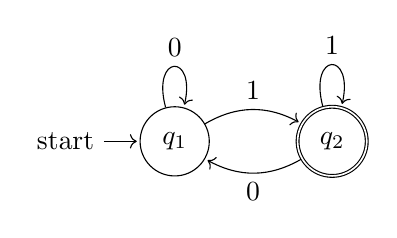
\begin{tikzpicture}[shorten >=1pt,node distance=2cm,on grid,auto] 

		\node[state,initial] (q_1)   {$q_1$}; 
		\node[state, accepting] (q_2) [right=of q_1] {$q_2$}; 
		 \path[->] 
		 (q_1) edge [bend left] node  {1} (q_2)
			   edge [loop above] node {0} ()
		 (q_2) edge [bend left] node {0} (q_1) 
			   edge [loop above] node {1} ();
	 \end{tikzpicture}
	\caption{State diagram of a finite automaton}\label{fig:automaton}
\end{figure}

\paragraph{Definition} A \textbf{\emph{deterministic finite automaton}} \( M \)  is a 5-tuple \( (Q, \Sigma, \delta, q_0, F) \), where

\begin{enumerate}
	\item \( Q \) is a finite set called the \textbf{states},
	\item \( \Sigma \) is a finite set called the \textbf{alphabet},
	\item \( \delta: Q \times \Sigma \rightarrow Q \) is the \textbf{transition function},
	\item \( q_0 \in Q \) is the \textbf{start state}, and
	\item \( F \subseteq Q \) is the \textbf{set of accept states}.    
\end{enumerate}

The set \( A \)  of all strings that a machine \( M \) accepts is the \textbf{language} \( L(M) = A \)  of the machine. We say that \( M \) \emph{recognises} or \emph{accepts}  \( A \). If a machine accepts no strings, it still accepts one language --- the empty language \( \emptyset \).

The transition function can be mapped using a two-dimensional table as shown for the function \( Q \times \Sigma \rightarrow Q \) where \( Q = \{q_1, q_2 \} \)  in \autoref{tab:transitionfunc}.

\begin{table}
	% \renewcommand{\arraystretch}{2}
	\centering

	\begin{tabular}{@{}lll@{}}
	\toprule
				& \texttt{0} & \texttt{1} \\ \midrule
	\( \mathbf{q_1}  \)	& \( q_1 \) & \( q_2 \) \\
	\( \mathbf{q_2}  \)	& \( q_1 \) & \( q_2 \) \\ \bottomrule
	\end{tabular}
	\caption{Mapping a transition function}\label{tab:transitionfunc}
\end{table}

If a machine \( M \) has a start state that is also an accept state, the machine will accept the empty string \( \epsilon \).

\subsection{Non-deterministic Finite Automata}
A deterministic finite automaton (DFA) has key differences from a non-deterministic finite automaton (NFA):

\begin{enumerate}
	\item In a \textbf{DFA}, \emph{every state} has exactly \emph{one exiting transition} for \emph{each symbol} in the alphabet.
	\item In an \textbf{NFA}, states may have \emph{none, one or more exiting transitions} for some or all symbols of the alphabet, including the empty string \( \epsilon\). 
\end{enumerate}

\begin{figure}[ht]
	\centering
	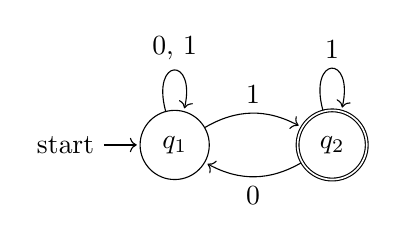
\begin{tikzpicture}[shorten >=1pt,node distance=2cm,on grid,auto] 

		\node[state,initial] (q_1)   {$q_1$}; 
		\node[state, accepting] (q_2) [right=of q_1] {$q_2$}; 
		 \path[->] 
		 (q_1) edge [bend left] node  {1} (q_2)
			   edge [loop above] node {0, 1} ()
		 (q_2) edge [bend left] node {0} (q_1) 
			   edge [loop above] node {1} ();
	 \end{tikzpicture}
	\caption{Example of a non-deterministic finite automaton}\label{fig:nfa}
\end{figure}

An example for an NFA is shown in \autoref{fig:nfa}.

An NFA computes by making copies of itself to pursue every possible option in parallel. Therefore, if a state has two transitions for a given symbol, the machine copies itself and follows both routes. If a transition is not possible, the machine dies and returns a reject state.

\paragraph{Definition} A \textbf{\emph{non-deterministic finite automaton} }  is a 5-tuple \( (Q, \Sigma, \delta, q_0, F) \), where

\begin{enumerate}
	\item \( Q \) is a finite set called the \textbf{states},
	\item \( \Sigma \) is a finite set called the \textbf{alphabet},
	\item \( \delta: Q \times \Sigma_\epsilon \rightarrow \mathcal{P}(Q) \) is the \textbf{transition function},
	\item \( q_0 \in Q \) is the \textbf{start state}, and
	\item \( F \subseteq Q \) is the \textbf{set of accept states}.    
\end{enumerate}

The \textbf{key difference} is the transition function, which maps the cross product of states and the alphabet, including the empty string \( \epsilon \), to a set of all possible next states, written as the power set of Q.

\section{Regular Languages}
A language is called a \textbf{regular language} if some finite automaton recognises it.

\subsection{Regular Operations}
Let \( A \) and \( B \) be languages. We define the regular operations \textbf{union}, \textbf{concatenation}, and \textbf{star} as follows:
\begin{enumerate}
	\item \textbf{Union}: \( A \cup B = \{x \mid x \in A \textrm{ or } x \in B \} \)
	\item \textbf{Concatenation}: \( A \circ B = \{xy \mid x \in A \textrm{ and } y \in B \} \)
	\item \textbf{Star}: \( A^{\star} = \{ x_1 x_2 \ldots x_k \mid k \geq 0 \textrm{ and each } x_i \in A\} \)  
\end{enumerate}

The \textbf{star} operation is a \textbf{unary} operator, in that it only operates on one alphabet. It takes all symbols from the alphabet and generates all possible  strings from language \( A \)  to form a new language \( A^* \). The empty string \( \epsilon \) is always a member of \( A^* \), as no string may be generated as one of the options.

Every NFA has an equivalent DFA in the sense that they both can recognise (accept) the same language.

A language is considered \emph{regular} if and only if at least one NFA accepts it. If two languages are \emph{regular}, then their \textbf{union}, \textbf{concatenation} and \textbf{star} are regular.

\subsection{Regular Expressions}

A \emph{regular expression} is a way to describe a language in a concise, general notation using regular operations.

The following is an example of a regular expression in shorthand notation and it's more expanded form.
 \[
(0 \cup 1)0^* = (\{0\} \cup \{1\})\circ \{0\}^*	
\]
In regular expressions, the order of precedence is given by \emph{star} \( \rightarrow \) \emph{concatenation} \( \rightarrow \) \emph{union}. Concatenation is implicit, meaning that is is assumed when no operator is given between two terms (as in the example above).

Say that \( R \) is a \textbf{regular expression} if \( R \) is

\begin{enumerate}
	\item \( a \) for some \( a \) in alphabet \( \Sigma \),
	\item \( \epsilon \),
	\item \( \emptyset \),
	\item (\( R_1 \cup R_2 \)), where \( R_1 \) and \( R_2 \) are regular expressions,
	\item (\( R_1 \circ R_2 \)), where \( R_1 \) where \( R_1 \) and \( R_2 \) are regular expressions, or
	\item (\( R_1^* \)), where \( R_1 \) is a regular expression.
\end{enumerate}

Don't confuse the regular expressions \( \epsilon \)  and \( \emptyset \). The expression \( \epsilon \)  represents the language containing a single string, the empty string. \( \emptyset \) describes the language that doesn't contain any strings.

\paragraph{Kleene's Theorem} A language is regular if and only if some regular expression describes it.

\subsection{Pumping Lemma}

If a language is not regular, then there is no DFA that recognises it. To prove that a language \( L \) is not regular, we can use a property of regular languages and prove non-regularity by contradiction.

A regular language can be \emph{pumped}, which means that with a sufficiently long input string, it cycles at least once. That means that a state in the automaton is visited twice (based on the pigeonhole principle). The \textbf{pumping lemma} states that such a string, while cycling one or more times, will still remain in the language.

\paragraph{Pumping Lemma} If \( A \) is a regular language, then there is a number \( p \) where if \( s \) is any string in \( A \) and \( s \leq p \) then \( s \) may be divided into three pieces \( s = xyz \) such that

\begin{enumerate}
	\item for each \( i \geq 0, xy^iz \in A \),
	\item \( |y| > 0 \), and
	\item \( |xy| \leq p \). 
\end{enumerate}

The first condition states that a string that has a cycling part remains in the language. The second part states that the cycling part may not be empty, it has to have at least one edge (meaning a node cycling onto itself). The this part states that the automaton needs to reach the start of the cycle before reaching the pumping length \(p\). 

The pumping lemma is only concerned with languages that generate very long (i.e.\ infinite strings).

\section{Context-Free Languages}

A grammar consists of \textbf{substitution rules} and describes how strings in a language are generated using such rules.

\paragraph{Definition} A \textbf{context-free grammar} is a 4-tuple \( (V, \Sigma, R, S) \) where

\begin{enumerate}
	\item \( V \) is a finite set called the \emph{\textbf{variables} },
	\item \( \Sigma \) is a finite set, disjoint from V, called the \textbf{\emph{terminals} },
	\item \( R \) is a finite set of \textbf{\emph{rules} }, with each rule being a variable and a string of variables and terminals, and
	\item	\( S \in V \) is the start variable.

	\paragraph{Example} The language \( L = \{o^n1^n\} \) can be described by the grammar \[
	S \rightarrow 0S1 \mid \epsilon	
	\]
	where \( S \) is the start variable, 0 and 1 are terminals and the entire statement is a substitution rule.
\end{enumerate}

\subsection{Chomsky Normal Form}
Any context-free grammar has an equivalent grammar in \textbf{Chomsky normal form} which is a simplified version that removes ambiguity from the grammar.

A context-free grammar is in \textbf{Chomsky normal form} if every production is of the form 
\begin{align*}
	A &\rightarrow BC \\
	A &\rightarrow a
\end{align*}
where \( a \) is any terminal and \( A, B, \) and \( C \) are any variables---except that \( B  \) and \( C \) may not be the start variable. In addition, we permit the rule \( S \rightarrow \epsilon \), where \( S \) is the start variable.

\paragraph{Converting to Chomsky normal form} The steps to convert a grammar to Chomsky normal form are given as follows.

\begin{enumerate}
	\item \textbf{Add a new start variable}  \( S_0 \) and the rule \( S_0 \rightarrow S \). This guarantees that the start variable occurs only on the left-hand side.
	\item \textbf{Remove all \( \epsilon \) rules \( A \rightarrow \epsilon \).}  For each occurrence of \( A \) on the right-hand side, add a new rule with that occurrence deleted.
	\item \textbf{Remove all unit rules}  of the form \( A \rightarrow B \). Replace all occurrences of \( B \) on the right-hand side with the terminal that is produced by \( A \). Eliminate the original unit rule.
	\item \textbf{Reduce any rules with more than two variables or more than one terminal}  to correct form. Replace variable pairs inside of n-tuples with new single variables and add corresponding rules. Replace any combinations of terminals and variables with variable pairs and add the corresponding rules.
\end{enumerate}




\section{Turing Machines}

A Turing machine is a more powerful model of a computer, similar to a finite automaton but with unlimited and unrestricted memory.

It consists of a control unit with a read/write head that moves along a tape which is divided into cells. The machine can move along the tape and read from or write to cells. The tape contains the input string at the beginning, followed by a space \( \sqcup \)  and an infinite amount of empty tape following it. Cells can be overwritten.

\paragraph{Definition} A \textbf{\emph{Turing machine} } is a 7-tuple \( (Q, \Sigma, \Gamma, \delta, q_0, q_{accept}, q_{reject}) \), where

\begin{enumerate}
	\item \( Q \) is a set of states,
	\item \( \Sigma \) is the input alphabet not containing the \textbf{blank symbol} \( \sqcup \) , 
	\item \( \Gamma  \) is the tape alphabet, where  \( \sqcup \in \Gamma \) and \( \Sigma \subseteq \Gamma \) 
	\item \( \delta: Q \times \Gamma \rightarrow Q \times \Gamma \times \{L, R\} \) is the transition function,
	\item \( q_0 \in Q \) is the start state,
	\item \( q_{accept} \in Q \) is the accept state, and
	\item \( q_{reject} \in Q\) is the reject state, where \( q_{reject} \neq q_{accept} \).     
\end{enumerate}

\paragraph{Configuration} A \emph{configuration} of a Turing machine describes it's current state, the current tape contents and the current head location. For a state \( q \) and two strings \( u\) and \( v \) over the tape alphabet \( \Gamma \), we write \( uqv \) for the configuration where the currents state is \( q \), the tape contents are \( uv \) and the head location is at the first symbol of \( v \). For example, \( \texttt{1011}q_7\texttt{01111} \) is the configuration where the current state is \( q_7 \), the tape contents are \texttt{101101111} and the current head location is at the second \texttt{0}. The \textbf{start configuration} of \( M \) on input \( w \) is the configuration \( q_0w \) which indicates the machine is in the start state \( q_0 \) and the head is at the leftmost position.

A Turing machine \( M \) \textbf{\emph{accepts} } input \( w \) if a sequence of configurations \( C_1, C_2, \ldots, C_k \) exists, where

\begin{enumerate}
	\item \( C_1 \) is the start configuration of \( M \) on input \( w \)
	\item each \( C_i \) yields \( C_{i+1} \), and
	\item \( C_k \) is an accepting configuration.
\end{enumerate}

The collection of strings that \( M \) accepts is the \textbf{language of} \( \mathbf{M} \). The language is \textbf{Turing-recognisable} if some Turing machine \emph{recognises} it. A Turing machine has three possible outcomes
	\begin{itemize}
		\item \emph{accept} 
		\item \emph{reject} 
		\item \emph{loop} 
	\end{itemize}
A Turing machine that never loops is called a \textbf{decider}. A language is \textbf{Turing-decidable} if some Turing machine \emph{decides} it.

\subsection{Halting Problem}
The \textbf{Halting Problem} is a kind of problem that cannot be solved by a Turing machine. Say we want to find out if a program \( P \) halts or loops for ever. No procedure exists to determine this, because if a program is still running after a fixed length of time, we do not know if it is still running or is looping forever. Hence we cannot computationally determine if the program will halt unless we let the program itself run to completion (or loop forever).
\section{Algorithms}

\subsection{Bubble Sort}
Bubble sort is popular, but inefficient, sorting algorithm. It works by repeatedly swapping adjacent elements that are out of order.

It starts at the head of a vector, compares the element to the adjacent elements, and swaps the elements if the first element is larger than the second element.

\paragraph{Passes} The Bubble sort algorithm may need multiple passes to sort the entire vector. The maximum number of passes is given by the most difficult vectors to solve - such that are completely in reverse order. In this case, the number of required passes is \( n-1 \) where \( n \) is the number of elements. Therefore, \textbf{the maximum number of passes required} is always \( n-1 \).  

\begin{algorithm}[H]
	\caption{Bubble Sort}\label{alg:bubble}
	\begin{algorithmic}
		\Function{Bubblesort}{\emph{vector}}
		\State{\( n \leftarrow\) LENGTH[\( vector \)] }
		\For{\( 1 \leq i \leq n-1 \) }
		\State{\( count \leftarrow 0\) }
		\For{\( 1 \leq j \leq n-1 \)}
		\If{\( vector[j+1] < vector[j] \) }
		\State{Swap(\(vector,j,j+1\))}
		\State{\( count \leftarrow count +1 \) }
		\EndIf{}
		\EndFor{}
		\If{\( count = 0 \) }
		\State{\textbf{break} }
		\EndIf{}
		\EndFor{}
		\State{\textbf{return} \emph{vector} }
		\EndFunction{}
	\end{algorithmic}
\end{algorithm}


\subsection{Insertion Sort}
Insertion sort works from the left of a vector, starting with the second element. It compares the element to the element on the left. If it needs to move, the element is moved along to the left as far as needed.

As an algorithm, we can store the current element in a temporary variable, while we ``move'' elements to the right by overwriting the slots to the right and then restoring the original values from the temporary variable.

\begin{algorithm}[H]
	\caption{Insertion Sort}\label{alg:insert}
	\begin{algorithmic}
		\Function{InsertionSort}{\emph{v}}
		\State{\( j \leftarrow 2 \) }
		\For{\( j \leq \) LENGTH[v]}
		\State{\( key \leftarrow v[j] \) }
		\State{\( i \leftarrow j - 1 \) }
		\While{\( i > 0 \wedge v[i] > key \) }
		\State{\( v[i+1] \leftarrow v[i] \) }
		\State{\( i \leftarrow i-1 \) }
		\EndWhile{}
		\State{\( v[i+1] \leftarrow key \) }
		\State{\( j \leftarrow j + 1 \) }
		\EndFor{}
		\EndFunction{}
	\end{algorithmic}
\end{algorithm}

\subsection{Binary Search}
Binary Search is a more efficient way of searching an item in a list. It proceeds by halving the list and comparing the middle element to the searched term. If the middle element is smaller than the term, the search continues on the right sublist, and if larger, on the left sublist. Then the procedure is repeated.

Binary search runs in logarithmic time \( O(log_{n}) \).

\begin{algorithm}[H]
	\caption{Binary Search}\label{alg:binary}
	\begin{algorithmic}
		\Function{BinarySearch}{\emph{v, item}}

		\State{\( L \leftarrow 1\) }
		\State{\( R \leftarrow\) LENGTH\([v]\)}
		\While{\( L \leq R \) }
		\State{\( M \leftarrow \lfloor{\frac{L+R}{2}}\rfloor{} \) }
		\If{\( v[M] < item \) }
		\State{\( L \leftarrow M+1 \) }
		\ElsIf{\( v[M] > item \) }
		\State{\( R \leftarrow M-1 \) }
		\Else{}
		\State{\textbf{return} \( M \) }
		\EndIf{}
		\EndWhile{}
		\State{\textbf{return} false}

		\EndFunction{}
	\end{algorithmic}
\end{algorithm}

Binary search is faster than linear search because each additional search step works on a smaller input (half of the previous input). Hence the time to complete one additional step decreases by half with each step. Hence the algorithm is logarithmic.

\subsection{Recursion}
Recursion is the concept of a procedure referring to itself recursively. The main applications for using recursion are
\begin{itemize}
	\item \textbf{Decrease and conquer}: Decreasing the problem to a \emph{base case} and calling a procedure recursively on every decreasing inputs until the base case is reached. 
	\item \textbf{Divide and conquer}: Split the problem into smaller partial problems and sort those first. 
\end{itemize}

\begin{algorithm}[H]
	\caption{Recursive decrease-and-conquer procedure}\label{alg:fact}
	\begin{algorithmic}
		\Function{Factorial}{\emph{n}}
		\If{\( n=0 \) }
		\State{\textbf{return} 1}
		\EndIf{}
		\State{\textbf{return} \textsc{Factorial}\(( n-1 )\)  }

		\EndFunction{}
	\end{algorithmic}
\end{algorithm}

\subsection{Quicksort}
Quicksort is a recursive algorithm to sort a vector. It partitions the vector into sub-vectors at an arbitrary pivot, and then moves the elements smaller than the pivot to the left of it and elements larger to the right, and then moves the pivot element to the correct location in the partition. It then repeats this process recursively on the sub-vectors.

While Quicksort has a worst-case time-complexity of \( \mathcal{O}(n^2) \), this case is unlikely to occur among possible inputs. The typical time complexity, or average-case complexity, is \( \mathcal{O}(n \log(n)) \)

\begin{algorithm}[H]
	\caption{Quicksort --- \( \mathcal{O}(n^2) \) }\label{alg:quick}
	\begin{algorithmic}
		\Function{Quicksort}{\emph{A, p, r}}
		\If{\( p < r \) }
		\State{\( q = \) \textsc{Partition}\( (A,p,r) \)  }
		\State{\textsc{Quicksort}\( (A,p,q-1) \) }
		\State{\textsc{Quicksort}\( (A,q+1,r) \) }
		\EndIf{}	
		\EndFunction{} \\
		\Function{Partition}{\emph{A,p,r}}
		\State{\( x \leftarrow A[r] \) } \Comment{Set the pivot to be the last element}
		\State{\( i \leftarrow p-1 \) } \Comment{Set \( i \) as the divider between elements smaller or bigger than \( x \) }
		\For{j = p \textbf{to} \( r-1 \) } \Comment{Loop through the vector}
		\If{\( A[j] \leq x\) }
		\State{\( i \leftarrow i+1 \) } \Comment{Move  divider to the right to include an element bigger than \( x \) }
		\State{exchange \( A[i] \)  with \( A[j] \) }  \Comment{Move the \( j \)th element to the left partition}
		\EndIf{}
		\EndFor{}
		\State{exchange \( A[i+1] \) with \( A[r] \)  } \Comment{Move the pivot to the right of the divider}
		\EndFunction{}
	\end{algorithmic}
\end{algorithm}

\subsection{Merge Sort}

Merge sort is another recursive algorithm that divides an array into subarrays, sorts them recursively and merges the resulting subarrays into an end result. This procedure relies on a \textsc{Merge} function that compares two stacks element-by-element and merges them by placing the smaller of two elements into the result stack first. This comparison is then done recursively on ever-smaller subarrays, until the subarray length is one. In order to simplify code, the version below places \emph{Sentinels} at the end of subarrays to terminate the comparison process and not have to track how many elements have been compared.

\begin{algorithm}
	\caption{Merge Sort --- \( \mathcal{O}(n \log n) \) }\label{alg:merge}
	\begin{algorithmic}
		\Function{Merge-Sort}{\emph{A,p,r} }
		\If{\( p < r \) }\Comment{Check if the array is longer than 1}
		\State{\( q \leftarrow \lfloor\frac{p+r}{2}\rfloor \) }
		\State{\textsc{Merge-Sort}\( (A,p,q) \) }
		\State{\textsc{Merge-Sort}\( (A,q+1,r) \) }
		\State{\textsc{Merge}\( (A,p,q,r) \) }
		\EndIf{}
		\EndFunction{}
		\\
		\Function{Merge}{\emph{A,p,q,r} }
		\State{\( n_1 \leftarrow q-p+1 \) } \Comment{Length of left subarray}
		\State{\( n_2 \leftarrow r-q \) } \Comment{Length of right subarray}
		\State{let \( L[1 \ldots n_1 + 1] \) and \( R[1 \ldots n_2 + 1] \) be new arrays  } \Comment{Extend length by 1 for sentinels}
		\For{\( i = 1 \)  \textbf{ to } \( n_1 \) } \Comment{Copy left subarray}
		\State{\( L[i] \leftarrow A[p+i-1]\) }
		\EndFor{}
		\For{\( j = 1 \)  \textbf{ to } \( n_2 \) } \Comment{Copy right subarray}
		\State{\( R[j] \leftarrow A[q+j]\) }
		\EndFor{}	
		\State{\( L[n_1 + 1] \leftarrow \infty \) } \Comment{Insert sentinels}
		\State{\( R[n_2 + 1] \leftarrow \infty\) }
		\State{\( i \leftarrow 1 \) }
		\State{\( j \leftarrow 1 \) }
		\For{\( k = p \) \textbf{ to } r }
		\If{\( L[i] \leq R[j]\) } \Comment{Pick left element}
		\State{\( A[k] \leftarrow L[i]\) }
		\State{\( i \leftarrow i + 1 \) }
		\Else{ \( A[k] \leftarrow R[j] \)} \Comment{Pick right element}
		\State{\( j \leftarrow j+1 \) }
		\EndIf{}
		\EndFor{}
		\EndFunction{}
	\end{algorithmic}
\end{algorithm}



\subsection{Gale-Shapley Algorithm}

The idea is to iterate through all free men while there is any free man available. Every free man goes to all women in his preference list according to the order. For every woman he goes to, he checks if the woman is free, if yes, they both become engaged. If the woman is not free, then the woman chooses either says no to him or dumps her current engagement according to her preference list. So an engagement done once can be broken if a woman gets better option.


\begin{algorithm}[H]
	\caption{Gale-Shapley Algorithm for Stable Matching --- \( \mathcal{O}(n^2) \) }\label{alg:gale}
	\begin{algorithmic}
		\Function{Gale-Shapley}{\emph{m,w,}, lists of preferences for each \emph{m, w}}
		\State{Initialize all women \( w \) and all men \( m \) to free}
		\While{\( \exists \) a free man \( m \) who still has a woman \( w \) to propose to}
		\State{ \( w \leftarrow m \)'s highest-ranked woman to whom he has not yet proposed }
		\If{\( w \) is free}
		\State{\( m,w \) become engaged}
		\Else{}
		\If{\( w \) prefers \( m \) to \( m' \) }
		\State{\( m, w \) become engaged}
		\State{\( m' \) becomes free}
		\Else{}
		\State{\( m',w \) remain engaged}
		\EndIf{}
		\EndIf{}
		\EndWhile{}
		\EndFunction{}
	\end{algorithmic}
\end{algorithm}

\section{Complexity Theory}

\subsection{Worst-Case Time Complexity}

Let \( M \) be a RAM machine that halts on all inputs. The \textbf{running time} or \textbf{time complexity} of \( M \) is the function \( f: N \rightarrow N \), where \( f(n) \) is the maximum number of steps that \( M \) uses on any input of length \( n \) . If \( f(n) \) is the running time of \( M \) , we say that \( M \) runs in time \( f(n) \) and that \( M \) is an \( f(n) \) time random access machine. Customarily we use \( n \) to represent the length of the input.

\subsubsection{Big-O Notation}
The \textbf{running time} of an algorithm on a particular input is the number of steps executed. Machine-independently, we define ``time-steps''. The total running time of an algorithm is defined as
\[
	\textrm{time cost per statement} \times \textrm{no. of executions per statement} = \textrm{total running time}
\]

Function growth can be described and compared using \textbf{Big-O Notation}. In \emph{asymptotic analysis}, we can consider only the highest order terms of a function and ignore the constants. For example, given the function \[
f(n) = 6n^3 + 2n^2 + 20n +45	
\]  

then the \emph{asymptotic} or \emph{Big-O} notation is given as 

\[
	f(n) = \mathcal{O}(n^3)
		\]  
	
A table of common functions and their respective Big-O notation is shown in \autoref{tab:bigo} and sorted by growth rate from slowest to fastest.

\begin{table}[ht]
	\centering
	\begin{tabular}{ll}
	\toprule
	\textbf{Type}  & \textbf{Notation} \\ \midrule
	Constant & \( \mathcal{O}(1) \) \\
	Logarithmic &  \(\mathcal{O}(\log(n)) =\mathcal{O}(\log(n^c))\) \\
	Polylogarithmic & \(\mathcal{O}((\log(n))^c) \) \\
	Linear & \(\mathcal{O}(n) \) \\
	Quadratic & \(\mathcal{O}(n^2) \)  \\
	Polynomial & \(\mathcal{O}(n^c) \) \\
	Exponential & \(\mathcal{O}(c^n) \) \\
	\bottomrule
	\end{tabular}
	\caption{Notation in Pseudocode}\label{tab:bigo}
	\end{table}

Formally, this means that any function is asymptotically \emph{upper-bounded} by its respective Big-O class.

Let \( f \) and \( g \) be functions. It holds that

\[
	\exists k \exists n_0 \forall n \{|f(n)| \leq k \cdot g(n) \mid k > 0, n > n_0  \} \implies f(n) \in \mathcal{O}(g(n))
\]
stating that the size of the function \( f(n) \) will eventually be overtaken by the Big-O class \( g(n) \) multiplied by a constant \( k \). It is an upper bound.

Because Big-O classes live inside each other, we always seek to ascertain the \emph{smallest} Big-O class in which a function exists.

\subsection{Summary of Sorting and Search Algorithms}
The worst-case and average-case time complexities are shown in 

\begin{table}[H]
	\centering
	\begin{tabular}{@{}lll@{}}
	\toprule
	\textbf{Algorithm}  & \textbf{Worst Case}  & \textbf{Average Case} \\ \midrule
	Bubble Sort & \( \mathcal{O}(n^2) \) & \( \Theta(n^2) \) \\
	Insertion Sort & \( \mathcal{O}(n^2) \) & \( \Theta(n^2) \) \\
	Quick Sort & \( \mathcal{O}(n^2) \) & \( \Theta(n \log(n)) \) \\
	Merge Sort & \( \mathcal{O}(n \log(n)) \) & \( \Theta(n \log(n)) \) \\
	Linear Search & \( \mathcal{O}(n) \) & \( \Theta(n) \) \\
	Binary Search &\( \mathcal{O}(\log(n)) \) & \( \Theta(\log(n)) \) \\
	\bottomrule
	\end{tabular}
	\end{table}

\subsection{Master Theorem}
In \emph{divide-and-conquer} problems, a recurrence relation can be used to state the problem. Suppose a problem of size \( n \) is divided into \( a \) subproblems each of size \( n/b \) where \( b \) is some integer greater than 1. Additionally, there is some additional work \( g(n) \) to be done in the \emph{combine} phase at the end of a divide-and-conquer routine (see CLRS). The recurrence relation can be then stated as \[
f(n) = af\big(\frac{n}{b}\big)+ g(n)
\]

where \( f(n) \) is the number of operations required to solve the problem of size \( n \).

The \textbf{master theorem} allows estimation of the size of functions that satisfy divide-and-conquer relations easily.

\begin{equation*}
	f(n) \text{ is } \begin{cases}
		\mathcal{O}(n^d) & \text{ if } a < b^d \text{,} \\
		\mathcal{O}(n^d \log n) & \text{ if } a = b^d \text{,} \\
		\mathcal{O}(n^{ \log_b a}) & \text{ if } a > b^d \\
	\end{cases}
\end{equation*}
\end{document}